% NOTE - this is only a template without real arguments
\begin{entry}{Measurement processor and Log Early Implementation}{Sep 2, 2021}
    \objective 
    
    Determine a data scheme for internal data (I.E. grid states and association data passed to the GO and logger.)
    Implement MCOutputLog
    Run a simulation and get output logs

    \outline

    \begin{itemize}
        \item Select data scheme (DICT OF DICTS)
        \item Add processing to EDMMeasurementProcessor
        \item Add accessor function to EDMMeasurementProcessor
        \item Write MCOutputLog
        \item Add accessor-logger routine to timekeeper
        \item Add log writing routine to timekeeper
        \item Add file closeout function to timekeeper closeout
        \item Test

    \end{itemize}

    \procedures
    
    See outline. Not much to add here. I'll come up with the test as I go along (see observations) since this is a
    pretty simple communication feedthrough in spite of how crucial it is to the system.

    \parameters
    
    N/A

    \observations

    Had a bunch of issues adding DER-EMs. A lot of them came from the fact that I was jumping back and forth between
    CIMHub and the Powergrid-Models repository. USE POWERGRID-MODELS FOR EVERYTHING. It grabs stuff from CIMHub, but the
    measurement stuff is in powergrid-models as well. Here is how the process works:

    \begin{enumerate}
        \item Create a text file containing the feeder ID and information about each DER. (See EGoT13\_der.txt in the
        powergrid-models/platform/DER folder.)
        \item Edit powergrid-models/platform/cimhubconfig.json to read "blazegraph\_url":
        "http://localhost:8889/bigdata/sparql".This was an issue for some reason.
        \item Edit powergrid-models/platform/DER/insert\_der.sh with the new filename. Run it. This will create a uuid
        file with IDs for the new DERs.
        \item Run the sparql query in the Data section below to verify DER-EMs have been added to the system.
        \item Edit/run powergrid-models/platform/list\_all\_measurements.sh
        \item Edit/run powergrid-models/platform/insert\_all\_measurements.sh
    \end{enumerate}


    \data
    
    \begin{verbatim}
        # Storage - DistStorage
        PREFIX r:  <http://www.w3.org/1999/02/22-rdf-syntax-ns#>
        PREFIX c:  <http://iec.ch/TC57/CIM100#>
        SELECT ?name ?bus ?ratedS ?ratedU ?ipu ?ratedE ?storedE ?state ?p ?q ?id ?fdrid (group_concat(distinct ?phs;separator="\n") as ?phases) WHERE {
         ?s r:type c:BatteryUnit.
         ?s c:IdentifiedObject.name ?name.
         ?pec c:PowerElectronicsConnection.PowerElectronicsUnit ?s.
        # feeder selection options - if all commented out, query matches all feeders
        #VALUES ?fdrid {"_C1C3E687-6FFD-C753-582B-632A27E28507"}  # 123 bus
        VALUES ?fdrid {"_49AD8E07-3BF9-A4E2-CB8F-C3722F837B62"}  # 13 bus
        #VALUES ?fdrid {"_5B816B93-7A5F-B64C-8460-47C17D6E4B0F"}  # 13 bus assets
        #VALUES ?fdrid {"_4F76A5F9-271D-9EB8-5E31-AA362D86F2C3"}  # 8500 node
        #VALUES ?fdrid {"_67AB291F-DCCD-31B7-B499-338206B9828F"}  # J1
        #VALUES ?fdrid {"_9CE150A8-8CC5-A0F9-B67E-BBD8C79D3095"}  # R2 12.47 3
         ?pec c:Equipment.EquipmentContainer ?fdr.
         ?fdr c:IdentifiedObject.mRID ?fdrid.
         ?pec c:PowerElectronicsConnection.ratedS ?ratedS.
         ?pec c:PowerElectronicsConnection.ratedU ?ratedU.
         ?pec c:PowerElectronicsConnection.maxIFault ?ipu.
         ?s c:BatteryUnit.ratedE ?ratedE.
         ?s c:BatteryUnit.storedE ?storedE.
         ?s c:BatteryUnit.batteryState ?stateraw.
           bind(strafter(str(?stateraw),"BatteryState.") as ?state)
         ?pec c:PowerElectronicsConnection.p ?p.
         ?pec c:PowerElectronicsConnection.q ?q.
         OPTIONAL {?pecp c:PowerElectronicsConnectionPhase.PowerElectronicsConnection ?pec.
         ?pecp c:PowerElectronicsConnectionPhase.phase ?phsraw.
           bind(strafter(str(?phsraw),"SinglePhaseKind.") as ?phs) }
         bind(strafter(str(?s),"#_") as ?id).
         ?t c:Terminal.ConductingEquipment ?pec.
         ?t c:Terminal.ConnectivityNode ?cn.
         ?cn c:IdentifiedObject.name ?bus
        }
        GROUP by ?name ?bus ?ratedS ?ratedU ?ipu ?ratedE ?storedE ?state ?p ?q ?id ?fdrid
        ORDER by ?name
    \end{verbatim}

    \results
    


\end{entry}


%\begin{entry}{CMake Error running EGOT-DCM Dockerfile}{Dec 02, 2020}
%    \objective
%
%    Determine the cause of the CMake error while running the dockerfile and modify file to get it to successfully build.
%
%    \outline
%
%    \begin{itemize}
%        \item Try running to see if it was just Lorry or a machine issue.
%        \item If it is a machine issue, modify configurations to ensure interoperability.
%        \item If I get the error track down its cause and modify dockerfile to fix.
%        \item Repeat until all builds are successful.
%    \end{itemize}
%
%    \procedures
%
%    \begin{itemize}
%        \item \mint{console}|git clone https://github.com/EGoT-DCS-SunSpec-Modbus|
%        \item \mint{console}|docker build -f Dockerfile.buster -t egot-dcs .|
%        \item \mint{console}|docker container run -i egot-dcs|
%    \end{itemize}
%
%    \observations
%
%    \begin{error}{Cmake Error: No CMAKE\_CXX\_COMPILER found}
%        \begin{figure}[H]
%            \centering
%            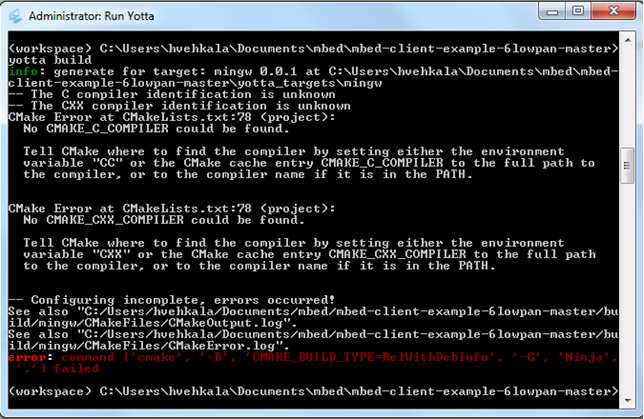
\includegraphics[height=4in]{Fall2020/Figures/cmake_error.png}
%        \end{figure}
%
%        Solution: what you need to do found at \cite{CMAKE-Forum}
%    \end{error}
%
%    \results
%
%    Short: No.
%
%    Long: Well...
%
%
%\end{entry}